\documentclass{article}
\usepackage{amsmath}
\usepackage{graphicx}
\usepackage{hyperref}
\usepackage{geometry}
\usepackage{cite}
\geometry{a4paper, margin=1in}

\title{Emotion Detection via EEG Signals by MATLAB}
\author{Asmaa Nasr}
\date{\today}

\begin{document}

\maketitle

\begin{abstract}
This report presents a methodology for detecting/recognition of emotions (happy, sad, fear, calm) using EEG signals processed in MATLAB. The approach includes data loading, filtering, normalization, feature extraction using Mel-frequency cepstral coefficients (MFCC), and classification using the k-nearest neighbors (KNN) algorithm. The model achieved an accuracy of 99.45\%.
\end{abstract}

\section{Introduction}
Emotion detection plays a crucial role in various applications, including human-computer interaction and mental health monitoring [1]. EEG signals provide valuable insights into emotional states. This report outlines a systematic approach to detect emotions based on EEG signals.

\section{Methodology}
The methodology includes:
\begin{enumerate}
\item Data Loading.
\item Data Filtering and Normalizing.
\item Feature Extraction by MFCC.
\item Classification by KNN.
\item Performance Validation using perfomance metrics.
\end{enumerate}
\subsection{Data Loading}
The first step involves loading the EEG data into MATLAB. The dataset consists of 4 recorded EEG signals (.mat) corresponding to different emotional states. 

\subsection{Filtering and Normalization}
Preprocessing is essential to remove noise and artifacts from the EEG signals. A band-pass filter is applied, followed by normalization.
The results are as shown in Figures 1-4.


Figure 1 shows fear EEG signal before and after Filtering.
\begin{figure}[htbp]
    \centering
    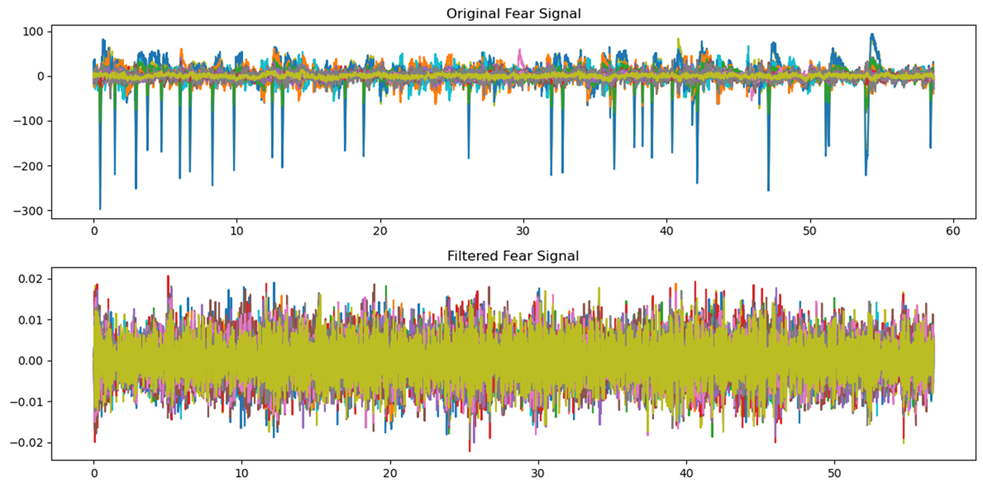
\includegraphics[width=0.8\textwidth]{f_fear.png}
    \caption{Fear Signal before and after filtering}
    \label{fig:fear}
\end{figure}

Figure 2 shows sad EEG signal before and after Filtering.
\begin{figure}[htbp]
    \centering
    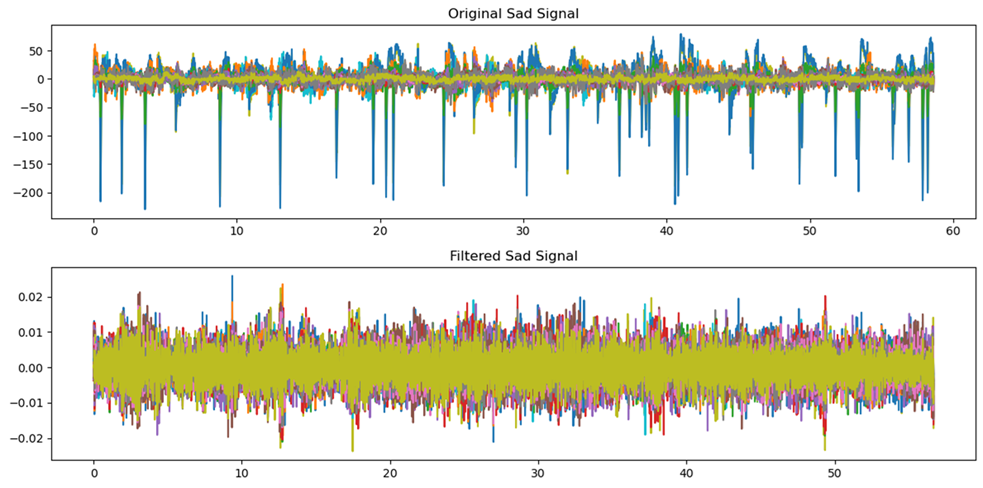
\includegraphics[width=0.8\textwidth]{f_sad.png}
    \caption{Sad Signal before and after filtering}
    \label{fig:sad}
\end{figure}

Figure 3 shows happy EEG signal before and after Filtering.
\begin{figure}[htbp]
    \centering
    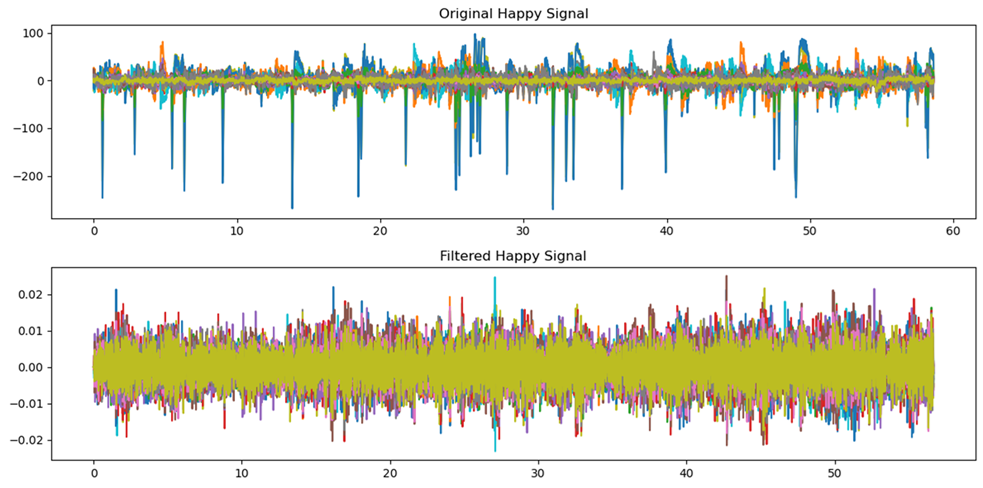
\includegraphics[width=0.8\textwidth]{f_happy.png}
    \caption{Happy Signal before and after filtering}
    \label{fig:happy}
\end{figure}

Figure 4 shows calm EEG signal before and after Filtering.
\begin{figure}[htbp]
    \centering
    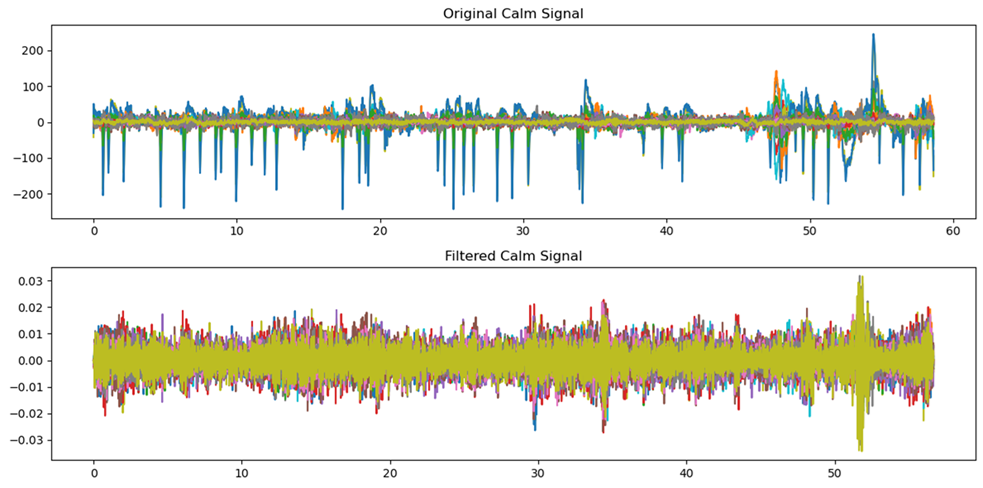
\includegraphics[width=0.8\textwidth]{f_calm.png}
    \caption{Calm Signal before and after filtering}
    \label{fig:calm}
\end{figure}


\subsection{Feature Extraction}
Mel-frequency cepstral coefficients (MFCC) are extracted to represent the emotional features of each channel individually and then combining the resulting features back together.
Features Extracted are 230 instances and 138 features. (230, 138)

\begin{verbatim}
% Feature extraction using MFCC
c_FP1=melcepst(Channel,fs,'M',nc,p,n,inc);
\end{verbatim}

\subsection{Classification using KNN}
The extracted features are classified using the KNN algorithm. The model is trained on a portion of the data (80\%) and tested on the remaining data (20\%).

\begin{verbatim}
% KNN classification
mdl = fitcknn(trainS, tgTrainS, 'NumNeighbors', 5);
predictions = predict(mdlx, testS);

% Calculate accuracy
accuracy = sum(predictions == tgTestS) / length(tgTestS) * 100;
% Confusion matrix
cm = confusionmat(tgTestS, predictions);

% Display the confusion matrix
disp('Confusion Matrix:');
disp(cm);
\end{verbatim}
\subsection{Classification Metrics}
\begin{enumerate}

\item The confusion matrix for the classification model provides insights into the model's performance across different emotional states. The diagonal elements represent the number of correct predictions for each emotion, while the off-diagonal elements indicate misclassifications [2].
\item To evaluate the model's performance, 5-fold cross-validation was employed. This method involves dividing the dataset into five subsets, or "folds" [3].
\end{enumerate}

\section{Results}
The model is trained on four folds and tested on the remaining one, and this process is repeated five times, ensuring that each fold serves as a test set once.
The cross-validation results provide a more robust estimate of the model's accuracy and help mitigate overfitting. Figures 5-9 shows the accuracy obtained for each fold during the validation process. The model consistently performed well across all folds, confirming its reliability.

\begin{figure}[htbp]
    \centering
    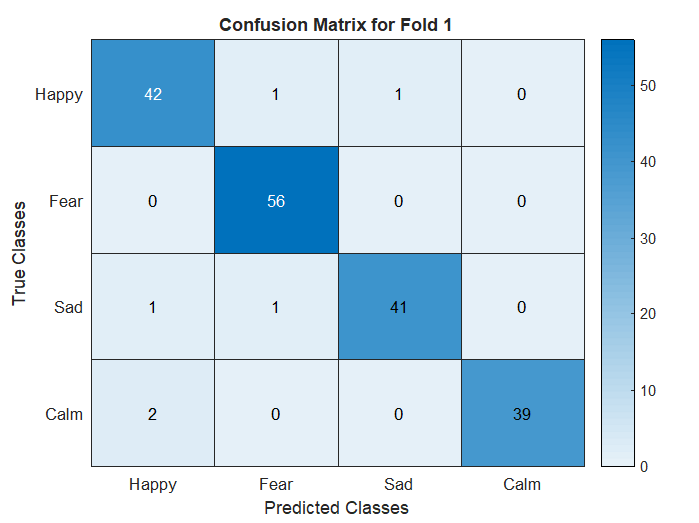
\includegraphics[width=0.6\textwidth]{cm1.png}
    \caption{Confusion Matrix of the 1st fold}
    \label{fig:cm1}
\end{figure}
\begin{figure}[htbp]
    \centering
    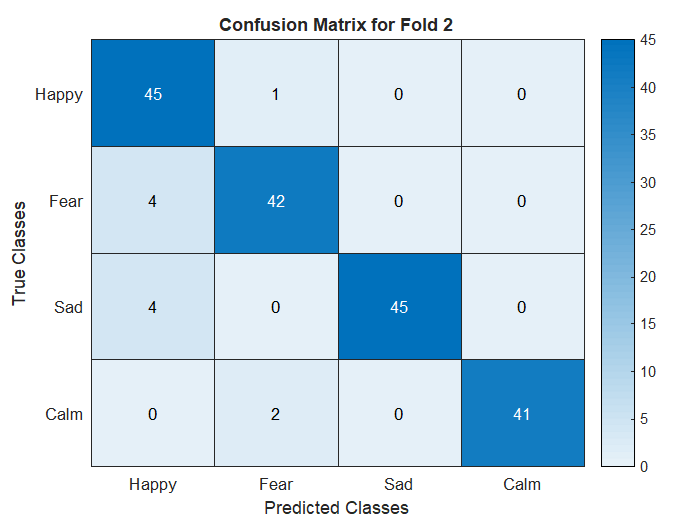
\includegraphics[width=0.6\textwidth]{cm2.png}
    \caption{Confusion Matrix of the 2nd fold}
    \label{fig:cm2}
\end{figure}
\begin{figure}[htbp]
    \centering
    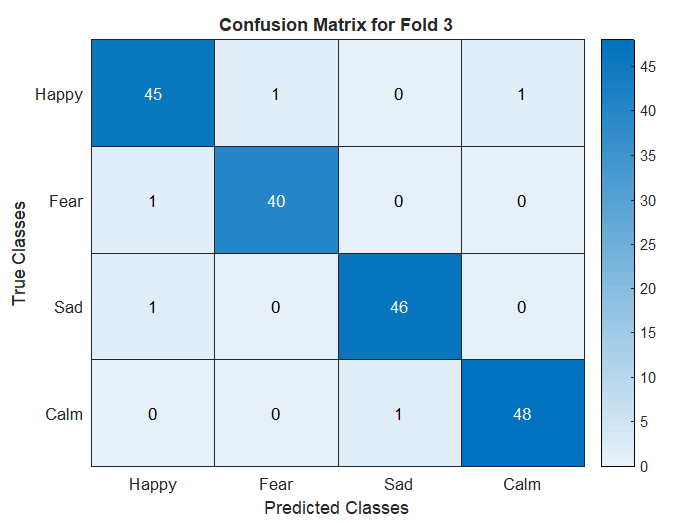
\includegraphics[width=0.6\textwidth]{cm3.png}
    \caption{Confusion Matrix of the 3rd fold}
    \label{fig:cm3}
\end{figure}
\begin{figure}[htbp]
    \centering
    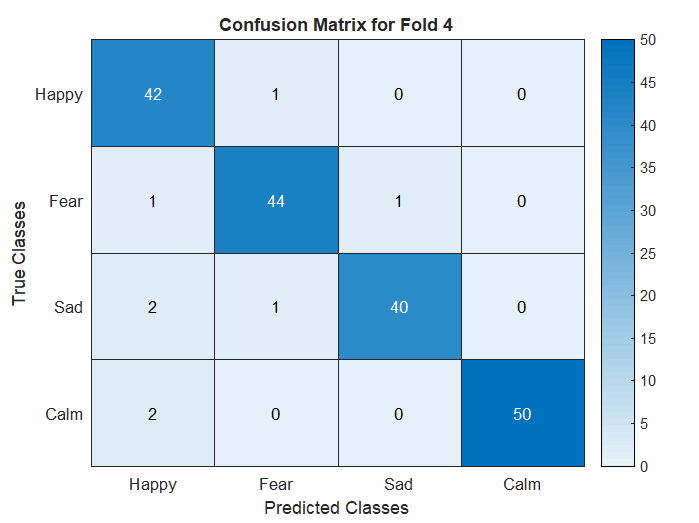
\includegraphics[width=0.6\textwidth]{cm4.png}
    \caption{Confusion Matrix of the KNN 4th fold}
    \label{fig:cm4}
\end{figure}
\begin{figure}[htbp]
    \centering
    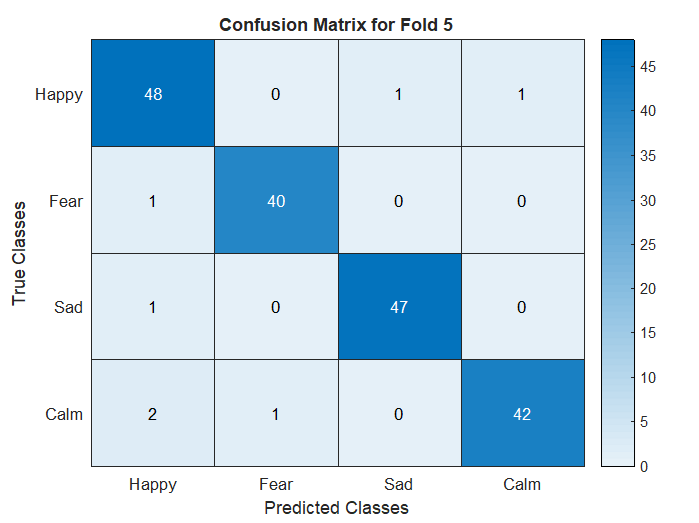
\includegraphics[width=0.6\textwidth]{cm5.png}
    \caption{Confusion Matrix of the 5th fold}
    \label{fig:cm5}
\end{figure}
The confusion matrix reveals that the model achieved high precision and recall for all emotional categories, further validating its effectiveness in emotion detection.
Figure 10 shows the overall confusion matrix of the model.

The KNN classifier achieved an accuracy of 99.45\% in detecting emotions from EEG signals, demonstrating the effectiveness of the proposed methodology.
\begin{figure}[htbp]
    \centering
    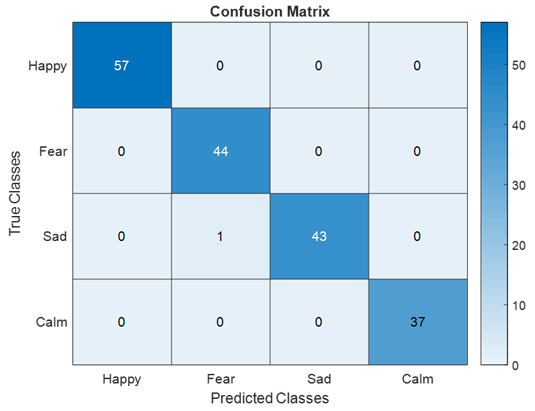
\includegraphics[width=0.6\textwidth]{Confusion_matrix.png}
    \caption{the overall Confusion Matrix}
    \label{fig:cm}
\end{figure}

\section{Conclusion}
The study successfully demonstrates the potential of using EEG signals for emotion detection. The combination of filtering, normalization, MFCC feature extraction, and KNN classification yielded high accuracy, making it a promising approach for further research.

\section{References}
\begin{thebibliography}{9}
\bibitem{b1} Houssein, E.H., Hammad, A., \& Ali, A.A. (2022). Human emotion recognition from EEG-based brain–computer interface using machine learning: a comprehensive review. \textit{Neural Computing and Applications}, 34, 12527–12557.\url{https://doi.org/10.1007/s00521-022-07292-4}.


\bibitem{b2} Malviya, N. (2023, April 19). Confusion matrix. Medium. \url{https://medium.com/@nikitamalviya/confusion-matrix-870739a1ec31}.

\bibitem{b3} Scikit-learn developers. (2025). Cross-validation: Evaluating estimator performance. In *Scikit-learn* (Version 1.7.1). Retrieved from \url{https://scikit-learn.org/stable/modules/cross_validation.html}.

\end{thebibliography}


\end{document}
